



\chapter{Background of the Virtual Heliodon System}
A tangible user interface is being developed in the computer graphics lab here at RPI.  This interface allows architects to design rooms within a new architectural space in a tangible way.  During this prototyping process architects can also experiment with lighting.  This architectural tool has been developed both in a small scale and a a full scale version.
\section{Tabletop Virtual Heliodon}
\label{tabletop}
Natural lighting is an often neglected issue when designing architecture.  Often buildings are originally designed only to client specifications and only when a design nears completion is lighting taken into account.  This results in many buildings using almost exclusively artificial lighting in the final design.  The graphics lab here at RPI created a tool has created a tool called the Virtual Heliodon to address this problem. The Virtual Heliodon \cite{ShengYYC09} is an architectural daylighting tool that continues to be improved in the RPI Computer Science Graphics Lab. 
 
A traditional heliodon uses a previously created architectural model or a model created specifically for this purpose.  The heliodon is comprised of a light and a rotating table.  The table or light above the table can be rotated such that different times of the day can be simulated by the directed light acting as a simulated sun.  Because of the time requirements of using such a system, traditional heliodons are not frequently used. The virtual heliodon is simpler to use in the design because it has a sketching interface complete with lighting simulation.

The Virtual Heliodon is a system in which foam core wall primitives can be moved around on a table top in order to design various spaces within a building.  The orientation can be specified with a \emph{north arrow primitive} and windows within this space can be specified by \emph{window primitives} which can be slid onto the top of the walls.  Computer vision techniques are used on images taken from an overhead camera to discover the geometry.  This geometry is then converted into a triangle mesh.  A patch based lighting method, radiosity, is used to simulate the light in the space.  The rendering system displays the simulated natural lighting in the room using six projectors spaced approximately equal distances from each other around the perimeter of the table.

The wall primitives used on the tabletop are rectangular pieces of foam core with cardboard feet attached to the bottom allowing them to stand up.  Three different heights of walls are available in the system; these heights are differentiated by distinct colors for each wall height.  A camera is mounted approximately seven feet above the tabletop. Because all of the primitives' heights can be inferred from the color of the walls, it is possible to completely reconstruct the room based only on the color of the walls and a single camera.  Window markers (made of colored pieces of index cards) can be fitted over the tops of walls to indicate where windows are desired.  The system has two different colored window markers allowing the user to specify and differentiate multiple instances of two types of windows.  In addition, a few unique markers have been developed to indicated traits such as the color of the walls, floor, and ceiling.  The position of these tokens does not matter because they are describing traits that apply to the whole scene.  The exception is the individual wall color markers which are associated with the nearest wall on the plane of the table.
\begin{figure*}[t]
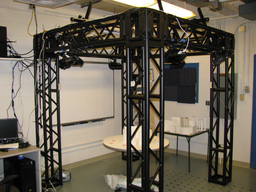
\includegraphics[width=0.5\textwidth]{images/IMG_1316.png}
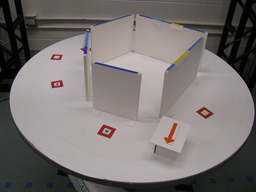
\includegraphics[width=0.5\textwidth]{images/IMG_1318.png}
\vspace{0.1in}\\
\begin{minipage}{0.5\textwidth}\vspace{-0.25in} \begin{center} Daylighting Tool Set-up \end{center}\end{minipage}%
\begin{minipage}{0.5\textwidth}\vspace{-0.25in} \begin{center} Example Primitives: note the walls, window markers and north arrow \end{center}\end{minipage}%
\vspace{-0.1in}
\caption{Tabletop Virtual Heliodon images}

\end{figure*}










